\documentclass [12pt]{report}
  \usepackage{listings}
  \usepackage{color}
  \definecolor{lightgray}{rgb}{.9,.9,.9}
  \definecolor{darkgray}{rgb}{.4,.4,.4}
  \definecolor{purple}{rgb}{0.65, 0.12, 0.82}
  \usepackage{graphicx}
  \usepackage{float}
  \usepackage{listings, xcolor}
  \definecolor{verylightgray}{rgb}{.97,.97,.97}
  \lstdefinelanguage{Solidity}{
    keywords=[1]{anonymous, assembly, assert, balance, break, call, callcode, case, catch, class, constant, continue, contract, debugger, default, delegatecall, delete, do, else, emit, event, export, external, false, finally, for, function, gas, if, implements, import, in, indexed, instanceof, interface, internal, is, length, library, log0, log1, log2, log3, log4, memory, modifier, new, payable, pragma, private, protected, public, pure, push, require, return, returns, revert, selfdestruct, send, storage, struct, suicide, super, switch, then, this, throw, transfer, true, try, typeof, using, value, view, while, with, addmod, ecrecover, keccak256, mulmod, ripemd160, sha256, sha3}, % generic keywords including crypto operations
    keywordstyle=[1]\color{blue}\bfseries,
    keywords=[2]{address, bool, byte, bytes, bytes1, bytes2, bytes3, bytes4, bytes5, bytes6, bytes7, bytes8, bytes9, bytes10, bytes11, bytes12, bytes13, bytes14, bytes15, bytes16, bytes17, bytes18, bytes19, bytes20, bytes21, bytes22, bytes23, bytes24, bytes25, bytes26, bytes27, bytes28, bytes29, bytes30, bytes31, bytes32, enum, int, int8, int16, int24, int32, int40, int48, int56, int64, int72, int80, int88, int96, int104, int112, int120, int128, int136, int144, int152, int160, int168, int176, int184, int192, int200, int208, int216, int224, int232, int240, int248, int256, mapping, string, uint, uint8, uint16, uint24, uint32, uint40, uint48, uint56, uint64, uint72, uint80, uint88, uint96, uint104, uint112, uint120, uint128, uint136, uint144, uint152, uint160, uint168, uint176, uint184, uint192, uint200, uint208, uint216, uint224, uint232, uint240, uint248, uint256, var, void, ether, finney, szabo, wei, days, hours, minutes, seconds, weeks, years},	% types; money and time units
    keywordstyle=[2]\color{teal}\bfseries,
    keywords=[3]{block, blockhash, coinbase, difficulty, gaslimit, number, timestamp, msg, data, gas, sender, sig, value, now, tx, gasprice, origin},	% environment variables
    keywordstyle=[3]\color{violet}\bfseries,
    identifierstyle=\color{black},
    sensitive=false,
    comment=[l]{//},
    morecomment=[s]{/*}{*/},
    commentstyle=\color{gray}\ttfamily,
    stringstyle=\color{red}\ttfamily,
    morestring=[b]',
    morestring=[b]"
  }
  
  \lstset{
    language=Solidity,
    backgroundcolor=\color{verylightgray},
    extendedchars=true,
    basicstyle=\footnotesize\ttfamily,
    showstringspaces=false,
    showspaces=false,
    numbers=left,
    numberstyle=\footnotesize,
    numbersep=9pt,
    tabsize=2,
    breaklines=true,
    showtabs=false,
    captionpos=b
  }
  
\title{Distributed ledgers application in Science: Smart
Papers on the Ethereum}
\author{YixuanXu (yx5u17@ecs.soton.ac.uk)\\University of Southampton}

\begin{document}
\maketitle
\newpage
\tableofcontents
\newpage
\listoffigures
\newpage
\listoftables
\newpage
\begin{abstract}
	This work is all about \dots
\end{abstract}
\newpage
\chapter{Introduction}
\section{Project aim}
\paragraph{}Digitization and Web technologies are now changing the way of publishing and disseminating the knowledge.
It becomes more convenient and less expensive for people to access the knowledge. 
The knowledge creation process is more dynamic right now. 
Text/graphics/rich media can be changed quickly and easily while at the same time being available to all the audiences.
However, most of current methods of academic publication are static, that means, they cannot be revised over time\cite{heller2014dynamic}. 
Web technologies actually have the power to make it more dynamic but is currently underused. On the other hands, journals, publishers and funders fully control
the entire process of academic publishing. The view of authors who should also participate in the publishing process tends to be underrepresented. 
Despite that fact that the current academic publishing system is advance and productive, 
authors still want a more open and decentralize publishing process \cite{d2018authors}.
\paragraph{}In the past, the scholarly books were keeping improving and updating for the centuries by releasing the new editions. 
Mistakes would be corrected, new result would be added and feedbacks would be used for improvement. 
Revising books allowed author to keep track with novel development \cite{heller2014dynamic}. 
Many handbooks and schoolbooks have been revised over and over again, resulting massive amount of quality publications.
In the contrast to books, academic paper were a kind of snapshot of certain scientific knowledge. 
Most of them were just published once. If there is a new finding, usually a new articles need to be published. 
But this kind of process are currently under debate and development \cite{heller2014dynamic}. 
The number of authors who want a more open process in scientific publishing is increasing rapidly. 
When it comes to the traditional of academic publishing, 
publishers play an important role of filtering good research, rejecting papers 
without sufficient conclusions. 
They make their decisions based on the peer-review process which is fully controlled by themselves. 
Since this kind of peer-review process usually will take a significant amount of time and is one of the
main reason of delaying publications, researcher came up with a new idea of doing publishing. A initial version
will be firstly released, then it could be updated after receiving the feedbacks from pre-peer-review. 
All the version will be always available and the changes made in the pre-peer-review process will also be stored after the publishing of final version.
The model allows the tracking of the development of academic papers. 
This improvements make the process of publishing process more dynamic and flexible.
But, there are some vital problems that have been discussed under such models 
which is the mechanism to manage the interactions between authors and contributor in a trust way \cite{Khoe:1994:CML:2288694.2294265}.
How can authors make agreements with each other about which version should be available ?
How can authors determine their contributions to the papers in a unprejudiced way ? On the other hand,
the contributions of reviewers is ignored in this model.
\paragraph{}In last few years, Distributed Ledger Technology have attracted public attentions as 
the most advanced tool that can provide a decentralized solutions to manage the interaction 
between people that may not trust each other. 
It also could guarantee the security and consistence without the need for admin. 
The special tools which could achieve such functionality is called Smart Contract. For the questions about the publishing model,
Smart contract could be programed to help authors to making decision in a decentralized way. The aim of this project is trying to provide a prototype of decentralize application 
to help authors to manage their publish and their attribution agreements in a dynamic and trusted way. 
The application itself will use the blockchain technology \cite{buterin2013ethereum}, so nobody can fully control the whole process.
It could be more reliable than the current publishing system. 
The implementation will be evaluated by the cost of using such system. 
A detailed cost analysis and data visualization will also be presented.  
\section{Outline}
\paragraph{}In Section 2, firstly it will present some modern publishing systems based on the blockchain.  
Then a general background of blockchain will be presented. After that, 
a more specific description about the smart contract on Ethereum would be shown for the following part
\paragraph{}In Section 3, it would give detailed design of the application. 
By comparing the blockchain technology with the current Web technology, 
It should gives more clear explanation why blockchain is preferred for this project
\paragraph{}In Section 4, it will focus on the Implementation. 
All the important implementation details will be described here
\paragraph{}Section 5 demonstrate the cost of using the decentralize application. 
The analysis consists of the visualization and specific code review.
\paragraph{}Section 6 will discuss the advantage and disadvantage of the current implementation.
Potential improvement would also be covered in this section.
\paragraph{}Section 7 will give a summary about the project and conclusion.
\chapter{Background Research}
\section{Modern publishing models example}
\paragraph{}Because of the development of web technologies, 
several models have been provided based on the modern web technologies to improve the process of the academic publish, 
making authors manage and produce their works more easier. 
DEIP \cite{DEIP} is a platform that aimed at effective and 
fair distribution of resource allocated to scientific and research activities.
It proposed a community-driven models that encourage the open knowledge without restriction.
The users of this platform could be both author and reviewers and have free access to all the publications. 
All the records of reviews will be recorded and reviewers will be awarded by the decentralized protocol.
Scienceroot \cite{science} is another blockchain-based publishing platform, 
it tries to creating a scientific publishing model which will reward and sustain researchers instead of maximizing the publishers' profits 
by using a fully decentralized storage platform called IPFS \cite{benet2014ipfs}. 
The Pluto \cite{Pluto} is also a platform that is trying to help researchers to get funding in a decentralized ways. 
It also wants to establish a more proper evaluation index for the academic publications. 
The ideas of these kinds of platforms are really aggressive but inspiring. 
They are trying to give the power back to authors and reviewers and to make the knowledge more open and accessible to everyone.
It could be found that modern publishing system requires more transparent review process and more trustable collaborations between authors.
The current Blockchain technologis have huge potential in aspect of creating decentralized application. So it could be found that all of above platform are 
using the Ethereum \cite{buterin2013ethereum} as their core framework. 
\section{Blockchain}
\paragraph{Technology}
On its most basic level, 
the blockchain is a new kind of information technology 
which is the combination of encryption methods with distributed computing.
Satoshi Nakamoto \cite{nakamoto2008bitcoin} combine them to make new ways to create a model 
where a network of computers collaborate to maintain a shared and secure database. 
This database consists of a string of blocks each one a record of data 
that has been encrypted and given a unique identifier called a hash.
Mining computers on the network validate transactions, 
add them to the block they are trying to build, 
and then broadcast the completed block to other nodes 
so that all have a copy of the database. 
Because there is no centralized server to validate the transaction to the database,
the blockchain depends upon a distributed consensus algorithm. 
In order to make an entry on to the blockchain database, 
all the computers have to agree about its state 
so that no one computer can make an alteration without the consensus of all others.
Once completed, a block goes into the blockchain as a permanent record. Each time a block get completed, a new one will be created.
Countless number of block connect to each other, like links in a chain. The kind of data structure makes the transactions immutable.
Every block contains hash value that is dependent on the hash of the previous block, 
if one is changed than all the other blocks linked to it going forward will be altered.
This works to make the data entered tamper-proof. 
This model is the working mechanism of the first generation blockchain which is known as Bitcoin.
Its functionalities are mainly focused on the small data storage, which is the history of transactions.
Blockchain are trying to create a secured, trusted, 
shared database and they do this through encryption and hashing,
proof of work and network consensus. The hashing and linking of blocks 
makes it difficult to go back and change a previous block once entered. 
And the proof of work system intentionally makes it computationally more difficult to alter the database,
thus making it extremely difficult to change all the blocks. It leads to a distributed consensus mechanism so that even if someone did it,
it is almost impossible to convince others to accept as the valid record. The bitcoin blockchain is a very good proof of the stability of such system.
It now secure hundreds of billions of dollars using this method without the network having been hacked. 
What this technology enables is a database that is secure with automatic trust 
which is powered by open source community and encryption.
It is tamper proof, once information is put into the database it can not be altered. 
It is a shared database as many people would have a up-to-date copy so that all have a single source of truth.
Likewise, it is transparent, all the transactions and alteration made to the blockchain is visible to everyone.
\paragraph{Ethereum}
With in a few years,
the second generation of blockchain emerged design as a network on which developers could build applications. 
It is going to be more like a distributed virtual computer than just database.
This was made technically possible by the development of the Ethereum platform. 
Ethereum is an open-source, public, blockchain-based distributed computing platform featuring smart contract functionality.
It provides a decentralize Turing-complete virtual machine, which can execute computer programs using a global network of nodes.
Ethereum was initial described in a white paper by Vitalik Buterin \cite{buterin2013ethereum}. 
The system has been very successful attracting a large and dedicated community of developers, supports and enterprises.
The important contribution of Ethereum as the second generation of blockchain is that 
it worked to extend the capacity of the technology from primary
being a database to becoming more a general platform for running decentralized application and smart contracts.
As of 2018 Ethereum is largest and most popular platform for building distributed application. 
It has been a major step forward to become a global distributed computer, 
a massive globally distributed cloud computing platform upon which we can run any application at scale and speed,
with the assurance that it has the security, resilience and trustworthiness of today's blockchain.
\paragraph{}
By reviewing the blockchain technology, 
it is easy to find out that Ethereum is really powerful to
help authors to make agreements and set their outcomes in stone so that they cannot be later repudiated.
In \cite{Khoe:1994:CML:2288694.2294265}, 
the Smart Paper model is proposed to provide a collaborative platform 
that preserves a single version of the truth through the collaborative process. 
Authors will use the smart contract to publish their works and collaborate with others.
Once decision is made, smart contract will guarantee the result of decision won't be change by anyone.
All the versions and meta data about contributions will be safely stored on the Ethereum.
\chapter{Design}
For a traditional publish model, it could be described as \ref{model}.
\begin{figure}[H]
  \centering
  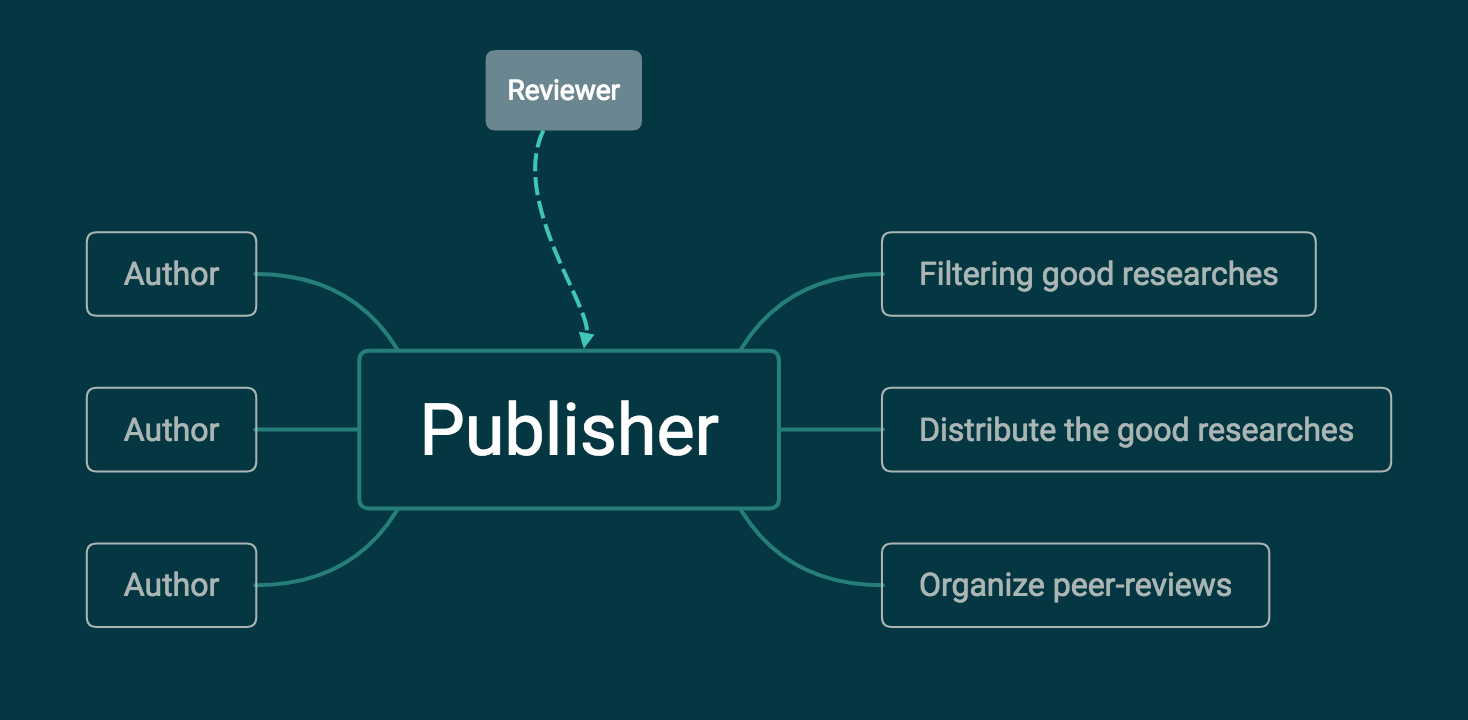
\includegraphics[width=0.9\textwidth]{traditionModel.png}
  \caption{Traditional publish model}
  \label{model}
\end{figure}
In this model, publishes takes all the responsibilities of filtering the good researches, 
rejecting papers with methods that are insufficient to draw the stated conclusion and the distributing widely\cite{heller2014dynamic}. 
The whole process is not transparent enough to the public.
It is vital to make everyone equal in this system.
\section{Requirements}
The first step of software developing is to identify the requirements from the specification,
then finding the correspond user cases.
The aim of this project is to provide a prototype of decentralize application 
to help authors to manage their publish and their attribution agreements.
Based on this, we could have these simple user cases:
\begin{itemize}
  \item Researchers should have their identities based on addresses of their Ethereum accounts
  \item Researchers should be able to use smart contract to publish a research artifacts, which will be represented by the hash of files
  \item Researchers should be able approve the contracts that belongs to themselves after verifying their local files with the online files with respect to a specific version
  \item The paper contracts should contains the description, metadata and version list of the research artifacts.
  \item The contents of papers could be update with the agreements of all authors. 
  \item New researchers could be added to an ongoing paper with the agreements of all the previous researchers.
  \item The application should be open sourced and decentralized. Anyone could deploy their own instances.
  \item The review process could be community-driven and powered by publisher.
\end{itemize}
\begin{figure}[H]
  \centering
  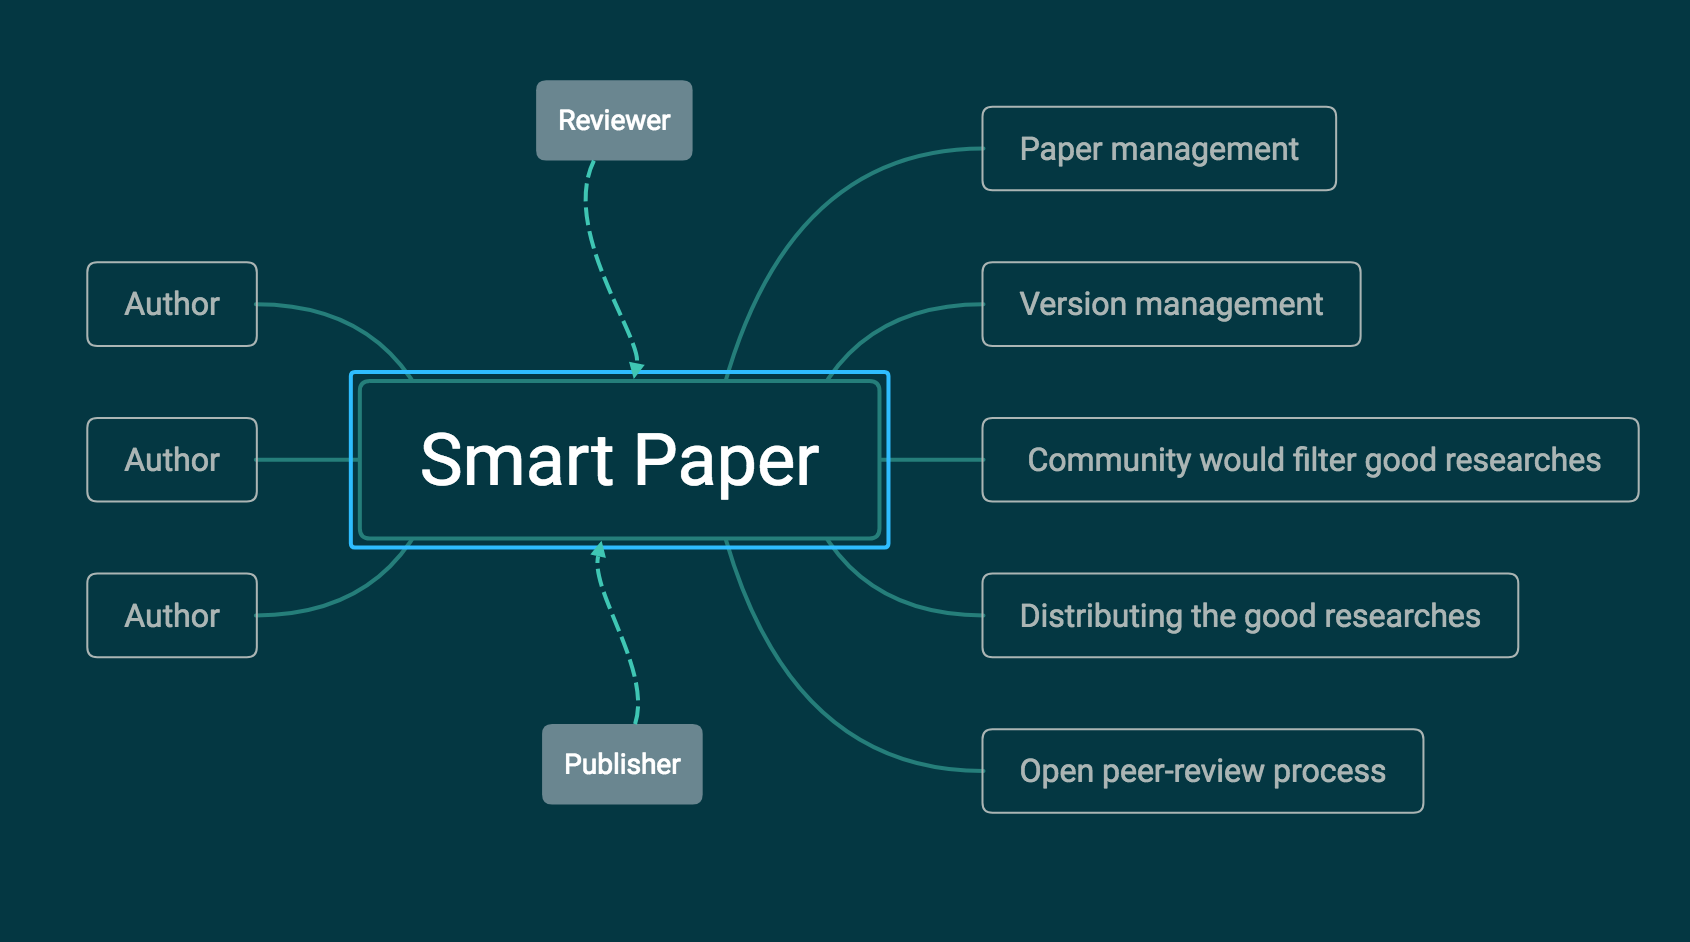
\includegraphics[width=0.9\textwidth]{smartPaperModel.png}
  \caption{Smart paper publish model}
  \label{smartPaper}
\end{figure}
The smart paper be design based these requirements. 
Based on the power of smart paper, we could have a new mechanism described as figure \ref{smartPaper}. 
In this model, the whole process of publishing would not be controlled by any individuals or organizations.
The smart paper consists of smart contracts which is used to implement those functionalities. 
\section{Smart Contract}
Three kinds of contracts, 
which are RBAC(Role based access control), smartPaper and smartPaperList, 
will be used in this project.
\begin{figure}[H]
  \centering
  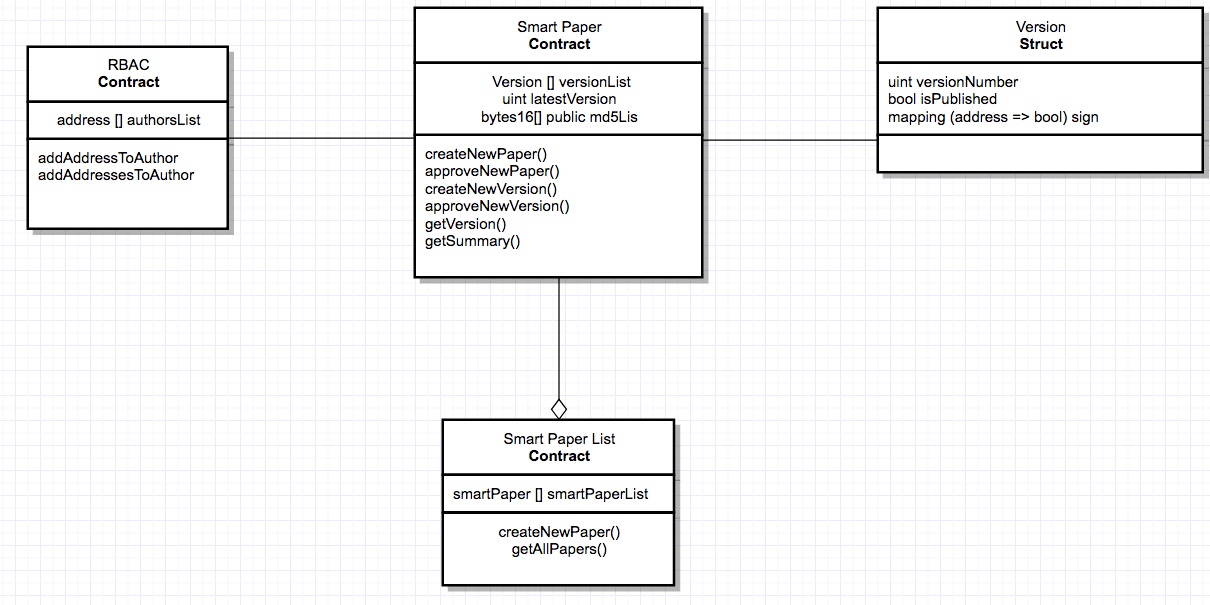
\includegraphics[width=1.0\textwidth]{uml.png}
  \caption{Smart Paper Design}
  \label{uml} 
\end{figure}
The initial design in design in \cite{Khoe:1994:CML:2288694.2294265} consider the single version of paper as a standalone contract.
However, it will increase the cost of smart paper. The current design is more cheaper by making the single version just a special data structure.
RBAC is a special contracts used for access managements. It maintain a hash table of the address of authors. 
Every time authors want to publish or approve a new version, 
RBAC will check the if authors belongs to this paper. 
Smart paper contains all the core functionalities, 
in the prototype application the hash of file will be stored instead of real file. The description and metadata will also stored in the contract.
Author can use the smart paper contract to publish new versions, then others authors need to approve the new version.
Once the new version is confirmed, 
it would be public available to the reviewers.  
The smart paper list contract is used to control all the smart paper and create new smart papers. 
It is the entry point of application.
\section{The Smart Paper workflow in Ethereum}
To begin with, a description of paper, metadata of paper, an array of addresses of authors and the file is submitted by a writer. 
The smart paper list will take those information and create a new smart paper contract which contains all the information. 
Then all the authors need to use the new smart paper contract to approve the initial version. Once a new version is finished, 
follow the same step, 
writer need to use smart paper contract to release a new version by providing the new description, metadata and file.
Then all the authors also need to approve the new version to make it public.
The smart paper workflow involves multiple working versions with dynamic collaborators. 
Version can become published and made available for annotating.
The smart paper list contract will keep the records of all the smart paper create by itself. 
User can access addresses of all the smart papers through this contract and check specific information of a paper by a specific address.
\chapter{Implementation}
\section{Technology Stack}
\section{Compiler deploy api testing}
\section{Client Development}
\section{Client Deployment}
\chapter{Evaluation}
\section{Cost analysis}
\section{Cost analysis design}
\section{Visualization}
\chapter{Discussion}
\section{Good}
\section{Bad}
\chapter{Conclusion}
\bibliographystyle{ieee}
\bibliography{ECS}
\end{document}
